\documentclass[12pt, a4paper]{scrartcl}

% !TeX root = ../ITS_WiSe_202021_Hausarbeit_969272.tex
\usepackage{a4wide}

\usepackage[utf8]{inputenc}

%\usepackage[ngerman]{babel}
\usepackage[english]{babel}

\usepackage[T1]{fontenc}
\usepackage{palatino}

\usepackage{graphicx}
\usepackage{caption}
\usepackage{url}
\usepackage{tocloft}
\usepackage{acronym}

\usepackage{mathpazo}
\usepackage{amsmath}
\usepackage{amsfonts}
\usepackage{adjustbox}

%\usepackage{subcaption}

\usepackage{hhline}
\usepackage{amssymb}
\usepackage{floatflt}
\usepackage{setspace}
\usepackage{float}
\usepackage{color}
\usepackage{listings}
\usepackage{array}
\usepackage{scrhack}
\usepackage{xcolor}
\usepackage{wrapfig}
\usepackage{hyperref}
\usepackage{url}
\usepackage{lmodern}
\usepackage{multirow}
\usepackage{subcaption}
\usepackage{cleveref}
\usepackage{lipsum}


% !TeX root = ../ITS_WiSe_202021_Hausarbeit_969272.tex
%%%%%%%%%%%%%%%%%%%%%%%%%%%%%%%%%%%%%%%%%%%%%%%%%%%%%%%%%%%%%%%%%%%%%%%%
% Data about you and the Document%
%%%%%%%%%%%%%%%%%%%%%%%%%%%%%%%%%%%%%%%%%%%%%%%%%%%%%%%%%%%%%%%%%%%%%%%%

% % Main Title of Document:
\newcommand{\myMaintitle}{ITS - Klausurersatzleistung}

% % Sub Title of DocInput:
\newcommand{\mySubtitle}{Developing holistic software solutions through integration of existing individual solutions.}

% % Ihr Name:
\newcommand{\myName}{Henrik Gerdes}

% % Matrikelnummer:
\newcommand{\myMatrikel}{MatNr: 969272}

% % Ihr Geburtsort:
\newcommand{\brith}{Osnabrück}

% % Ihr Geburtsort:
\newcommand{\place}{Osnabrück}

% % Ihr Abgabedatum:
\newcommand{\submission}{\today}

% % Ihr Abgabedatum:
\newcommand{\mycourse}{IT - Sicherheit}

% % Name des Betreuers/Erstprüfenden:
\newcommand{\fistSupervisor}{Dennis Ziegenhagen}
\newcommand{\secSupervisor}{Prof.\ Elke Pulvermüller}

% % In welchem Semester befinden Sie sich?
\newcommand{\mySemester}{6. Semester}

\title{\myMaintitle}

\author{\myName}
% !TeX root = ../ITS_WiSe_202021_Hausarbeit_969272.tex
% % Zeilenabstand im Haupttext auf anderthalb-zeilig setzen
%\linespread{1.25}\selectfont

% Line spacing
%\onehalfspacing{}

%Pfad für Grafiken
\graphicspath{{fig/}}

%Styleregeln
\widowpenalty10000 % Vermeidet einzelne Zeilen eines Absatzes zu Beginn einer Seite
\clubpenalty10000 % Vermeidet einzelne Zeilen eines Absatzes am Ende einer Seite
\addtocontents{toc}{\protect\sloppy}
\setcounter{tocdepth}{3}


% % \sloppy bewirkt, dass Latex beim Blocksatz nicht über den rechten Rand hinausschreibt.
% % und dafür größere Lücken in einer Zeile in Kauf nimmt
\sloppy

% % Setzt Dokumenteigenschaften für PDFs, wenn das Paket 'hyperref' geladen wurde.
\hypersetup{pdftitle=\myMaintitle,pdfauthor=\myName,bookmarksopen=true}

%Source for picture captions
\newcommand{\source}[1]{\caption*{Source: {#1}} }

\newcommand{\code}[1]{\texttt{#1}}

\newcommand{\myparagraph}[1]{\paragraph{#1}\mbox{}\\}

\newcommand{\RM}[1]{\MakeUppercase{\romannumeral{} #1{}}}

\newcommand{\HRule}{\rule{\linewidth}{0.5mm}} % Defines a new command for horizontal


\definecolor{dkgreen}{rgb}{0,0.6,0}
\definecolor{gray}{rgb}{0.5,0.5,0.5}
\definecolor{mauve}{rgb}{0.58,0,0.82}

\lstset{ %
  language=Java,                  % the language of the code
  basicstyle=\footnotesize,       % the size of the fonts that are used for the code
  numbers=left,                   % where to put the line-numbers
  numberstyle=\tiny\color{gray},  % the style that is used for the line-numbers
  stepnumber=1,                   % the step between two line-numbers. If it's 1, each line
                                  % will be numbered
  numbersep=5pt,                  % how far the line-numbers are from the code
  backgroundcolor=\color{white},  % choose the background color. You must add \usepackage{color}
  showspaces=false,               % show spaces adding particular underscores
  showstringspaces=false,         % underline spaces within strings
  showtabs=false,                 % show tabs within strings adding particular underscores
  frame=single,                   % adds a frame around the code
  rulecolor=\color{black},        % if not set, the frame-color may be changed on line-breaks within not-black text (e.g. commens (green here))
  tabsize=4,                      % sets default tabsize to 2 spaces
  captionpos=b,                   % sets the caption-position to bottom
  breaklines=true,                % sets automatic line breaking
  breakatwhitespace=false,        % sets if automatic breaks should only happen at whitespace
  title=\lstname,                 % show the filename of files included with \lstinputlisting;
                                  % also try caption instead of title
  keywordstyle=\color{blue},          % keyword style
  commentstyle=\color{dkgreen},       % comment style
  stringstyle=\color{mauve}         % string literal style
}

%%%%%%%%%%%%%%%%%%%%%%%%%%%%%%%%%%%%%%%%%%%%%%%%%%%%%%%%%%%%%%%%%%%%%%%%%%%%%%%%%%%%%%%%%
%Examples
%%%%%%%%%%%%%%%%%%%%%%%%%%%%%%%%%%%%%%%%%%%%%%%%%%%%%%%%%%%%%%%%%%%%%%%%%%%%%%%%%%%%%%%%%
% \pdfmarkupcomment[markup=Squiggly,color=green]{with pdfcomment}{move to the front}.
% \pdfmarkupcomment[markup=StrikeOut,color=red]{stupid}{replace stupid with funny}
% \pdfmarkupcomment[markup=Highlight,color=yellow]{Of course, you can highlight complete sentences.}{Highlight}
% \pdfcomment[icon=Note,color=blue]{insert graphic!}

\begin{document}

\pagenumbering{gobble}
% !TeX root = ../ITS_WiSe_202021_Hausarbeit_969272.tex
%%%%%%%%%%%%%%%%%%%%%%%%%%%%%%%%%%%%%%%%%
% Academic Title Page
% LaTeX Template
% Version 2.0 (17/7/17)
%
% This template was downloaded from:
% http://www.LaTeXTemplates.com
%
% Original author:
% WikiBooks (LaTeX - Title Creation) with modifications by:
% Vel (vel@latextemplates.com)
%
% License:
% CC BY-NC-SA 3.0 (http://creativecommons.org/licenses/by-nc-sa/3.0/)
%
% Instructions for using this template:
% This title page is capable of being compiled as is. This is not useful for
% including it in another document. To do this, you have two options:
%
% 1) Copy/paste everything between \begin{document} and \end{document}
% starting at \begin{titlepage} and paste this into another LaTeX file where you
% want your title page.
% OR
% 2) Remove everything outside the \begin{titlepage} and \end{titlepage}, rename
% this file and move it to the same directory as the LaTeX file you wish to add it to.
% Then add \input{./<new filename>.tex} to your LaTeX file where you want your
% title page.
%
%%%%%%%%%%%%%%%%%%%%%%%%%%%%%%%%%%%%%%%%%

%----------------------------------------------------------------------------------------
%	TITLE PAGE
%----------------------------------------------------------------------------------------
%Titelseite
\begin{titlepage}
	\centering
	\thispagestyle{empty}
	\begin{center}
	
\includegraphics[width=0.9\textwidth]{uos.pdf}
	\end{center}
	\LARGE{\textsc{Institut für Informatik\\Arbeitsgruppe Verteilte Systeme}}
	\vfill
	\HRule\\[0.4cm]
	\LARGE{\emph{\mycourse}}\\
	\vspace{8mm}
	\huge{\textbf{{\fontfamily{ppl}\selectfont
	\myMaintitle}}}\\
	\HRule\\[0.4cm]
	\vspace{9mm}
	\LARGE{\myName}\\
	\vspace{0.2cm}
	%ACHTUNG: !!!Matrikelnummer nur für die Abgabeversion, NICHT mit ins Wiki hochladen!!!
	\normalsize{\myMatrikel}\\
	\vspace{4cm}
	\large{Wintersemester}\\
	\vspace{0.2cm}
	\large{\today}
	\vfill
	\end{titlepage}
	\newpage


\tableofcontents
\newpage
\newcounter{lastroman}
\setcounter{lastroman}{\value{page}}

\pagestyle{plain}
\pagenumbering{arabic}
\maketitle

\section{Introduction}
Im Rahmen der Klausurersatzleistung für das Modul IT-Sicherheit wurde eine Proxy Client-Server Architektur erstellt mit der TCP Verbindungen umgeleitet werden können, um z.B. Filterregeln einer Firewall zu umgehen. Blockierte Anwendungen können dann den ProxyClient verwenden um dennoch nutzbar zu sein. Der strukturelle Aufbau is in fig \ref{fig::arch} zu sehen.\newline
Umgesetzt wurde diese Struktur indem Server und Client eine gemeinsame Tunnelklasse nutzen. Die Klasse Tunnel besteht aus einem \textit{SocketServer.TCPServer}, der bereits die unterliegenden sockets und den nicht blockierenden Programmablauf regelt sowie einem anwendungsspezifischen Handler der bei eintreffenden Anfragen aufgerufen wird. Server und Client haben jeweils einen eigenen Handler der die Kommunikation zwischen einander und zu den Endpunkten steuert. Es sind gleichzeitige Verbindungen möglich.

\begin{figure}[H]
    \centering
    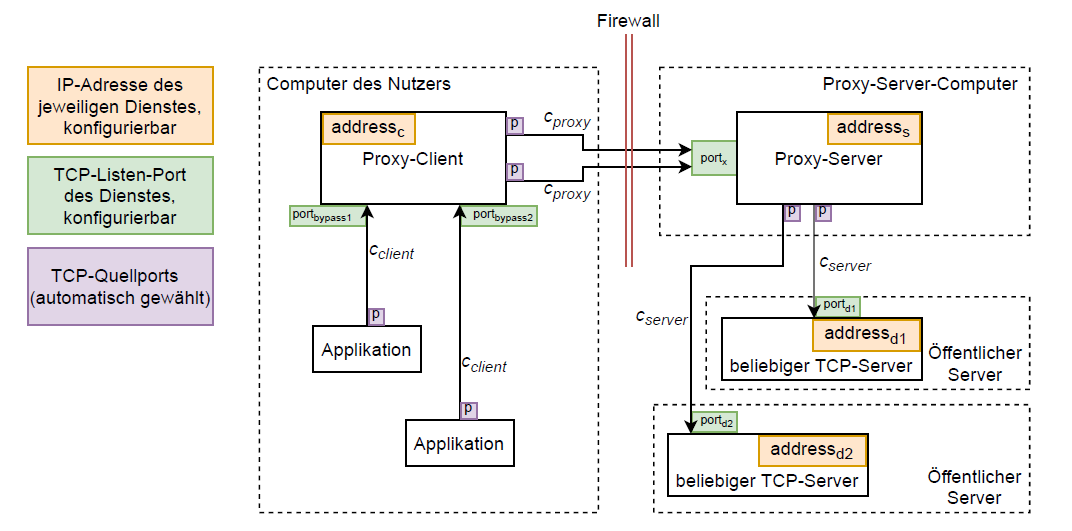
\includegraphics[width=0.9\textwidth]{structure.png}
    \caption{Netzwerk-Architektur zur Firewall-Umgehung}
    \label{fig::arch}
\end{figure}

\section{Security}
Nach Abschluss der Aufgabe 1 besteht eine funktionstüchtige Client-Server-Proxy Architektur. Diese unterliegt jedoch bestimmten Einschränkung hinsichtlich sicherer Nutzung. Diese Einschränkungen werden nachfolgend bearbeitet.
\subsection{Entitäten}
Die Nutzung kann auf folgende Entitäten aufgeteilt werden:
\begin{itemize}
    \item Anwender:
    \begin{itemize}
        \item Anwendung
        \item ProxyClient
    \end{itemize}
    \item Proxy-Betreiber
    \begin{itemize}
        \item ProxyServer
    \end{itemize}
    \item Inhaltsanbieter
    \begin{itemize}
        \item E-Mail
        \item WebDienste
        \item PrivateDienste
        \item \ldots
    \end{itemize}
\end{itemize}
Der nachfolgende Paragraph beschäftigt sich mit der Beziehung zwischen Anwender und Proxy-Betreiber
\subsection{Verletzte Grundprinzipien}
\paragraph{Anwender \& Betreiber:}
\noindent Der ProxyServer ist frei aus dem Internet erreichbar und nimmt von jedem anfragendem Dienst Datenpakete entgegen. Dabei kann der Server nicht Verifizieren, dass der anfragende Dienst tatsächlich der von Server erwartete ProxyClient ist. Dies verstößt gegen den Grundsatz der \textbf{Authentication}.\newline
Die Kommunikation zwischen ProxyClient und ProxyServer läuft über fremde Kommunikationswege. Jeder der Zugriff auf einen Teil dieses Kommunikationsweges hat kann die übertragenen Informationen mit Programmen wie Wireshark mitschneiden und möglicherweise gegen die Kommunikationspartner verwenden. Die Möglichkeit zum belauschen und lesen der Kommunikation verstößt gegen die \textbf{Confidentiality}.\newline
Neben dem mitlesen können die übertragenden Informationen auch verändert werden was gegen die \textbf{Integrity} verstößt.
\paragraph{Betreiber \& Inhaltsanbieter:}
Der ProxyServer Anbieter ermöglicht es fremden Entitäten seine Dienste zu nutzen sowie durch diese fremden Entitäten Anfragen an Dritte zu richten. Dabei trägt der ProxyServer Anbieter die Verantwortung für Angriffe oder andere Illegale Handlungen die über seine Infrastruktur gegenüber Dritte getätigt werden.\newline
Auch die eigene Infrastruktur kann Ziel eines Angriffs werden, indem z.B. Angreifer so viele Anfragen an der Proxy stellen, dass dieser zusammenbricht und nicht mehr durch andere genutzt werden kann, wie bei einem klassischen \ac{DoS} angriff.
\subsection{Lösungsansetze}
\section{Evaluation}


% Anhang
\newpage
\renewcommand{\thesubsection}{\Alph{subsection}}
\pagenumbering{Roman}
\setcounter{page}{\value{lastroman}}
\section*{Appendix}
\addcontentsline{toc}{section}{Appendix}
%Abkürzungsverzeichnis
% !TeX root = ../ITS_WiSe_202021_Hausarbeit_969272.tex
\newcommand{\abbr}{Abbreviations}
\subsection{Abbreviations}
%\addcontentsline{toc}{subsection}{Abbreviations}

\begin{acronym}[1234567890]		%[längste Abkürzung]
\setlength{\itemsep}{-\parsep}	% sorgt dafür, dass das Verzeichnis kompakt dargestellt wird.

\acro{DoS}[DoS]{Denial of Service}
\acro{TLS}[TLS]{Transport Layer Security}
\acro{HTTP}[HTTP]{Hypertext Transfer Protocol}
\acro{ACL}[ACL]{Access Control List}
\acro{SSL}[SSL]{Secure Sockets Layer}
\acro{VoIP}[VoIP]{Voice over IP}

\end{acronym}
\end{document}
